%!TEX program = xelatex
\documentclass[12pt, a4paper]{ctexart}

% \linespread{1.5}
\usepackage{geometry}
\usepackage{ctex}
\usepackage{tikz}
\usepackage{amsmath,amsfonts,amssymb,amsthm}
\usepackage{float}
\usepackage{enumerate}
\usepackage{fullpage}
\usepackage[ruled,linesnumbered]{algorithm2e}
\usepackage{hyperref}
\usepackage{listings} %代码块
\usepackage{graphicx}

\CTEXsetup[format={\Large\bfseries}]{section}
\geometry{a4paper,left=2.5cm,right=2.5cm,top=1.9cm,bottom=1.9cm}

\begin{document}
    \pagenumbering{arabic}         % 页码格式采用阿拉伯数字
    
    \title {\textbf{信息论与编码——信源编码实验}}
    \author{Harrison-1eo}
    \date{\today}
    \maketitle

\section{Huffman编码}
    \subsection{代码解释}
    在压缩过程中,首先统计输入数据中各个字节出现的频率,得到一个字典。然后根据频率构建哈夫曼树,对哈夫曼树的叶子结点进行编码,得到一个字典,键为字节,值为对应的编码。将编码后的数据按照 8 位一组进行分组,不足 8 位时在末尾补 0,并将分组后的每一组转换为一个字节,得到压缩后的数据。
    
    在解压缩过程中,首先对解压缩文件的头部信息进行解析,得到每个字节及其对应的频率信息。利用这些信息构建哈夫曼树,得到与压缩时相同的字典。然后将压缩文件中的 01 串按照 8 位一组进行分组,每组代表一个编码,利用哈夫曼树进行解码得到原始数据。最后将解压缩得到的原始数据输出。
    
    整个过程中使用了节点类(node)和哈夫曼树类(Huffman),并通过类方法的方式来进行代码组织,方便了代码的维护和扩展。

    Huffman压缩和解压缩过程中没有使用第三方包,由于使用了函数参数类型与返回值类型的注解,需要Python 3.x 版本。

    \subsection{码树的保存}
    在压缩过程中,首先统计各个字节出现的频率。将频率进行排序,并从小到大从0开始编号,这样256个字符最多需要256个数字表示,即编号最大不超过1字节。将每个出现的字节和对应的编号依次写入文件。在解码时,可以通过频率大小的顺序重新构建码树,进行解码。

    在这种保存方式下,码树的保存最差情况下(256个字节都出现过)需要占用512字节大小。

    \subsection{安全性和鲁棒性的考虑}
    由于我的程序设计为窗口程序打开文件,将读取到的文件内容以bytes类型提交给下一层的程序处理。因此对于空文件的输入,在打开文件时就会在上层提示打开的是一个空文件。同时还会判断待输入文件是否可读、路径是否存在等问题。

    对于单字符文件,在压缩阶段会判断字典长度是否为1,如果是,则将这唯一的字符编码为一个比特的0。在解码时,码树信息如果长度为2,则表示是一个单字符文件,解码时将后续所有的0解码为该字符。

    对于使用本程序编码得到的.enc文件,在第一行存储原文件的文件名和文件类型,便于解码过程的恢复,在第二行存储hu字符表示为Huffman编码得到的,并在之后存储其他数据。如果不符合这个格式规范,则会报错提示,此文件并非由本程序编码得到。

    \subsection{结果展示}
    \begin{figure}[H]
    \centering
    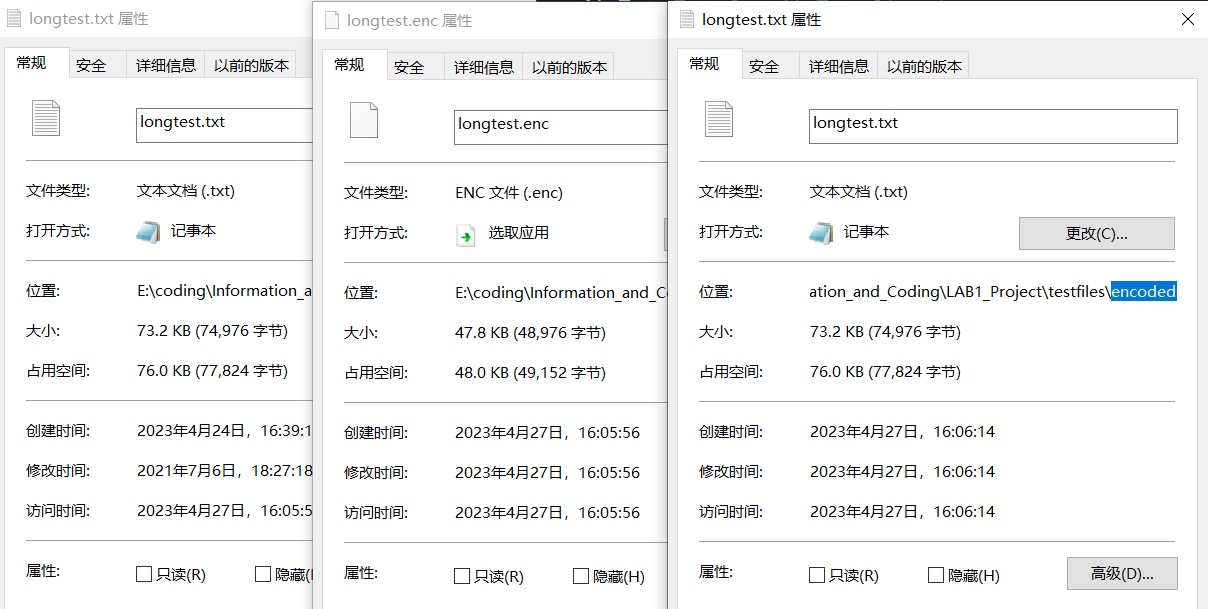
\includegraphics[width=10cm]{./pic/1-1.png}		
    \caption{Huffman编码longtest.txt}
    \end{figure}
    \begin{figure}[H]
    \centering
    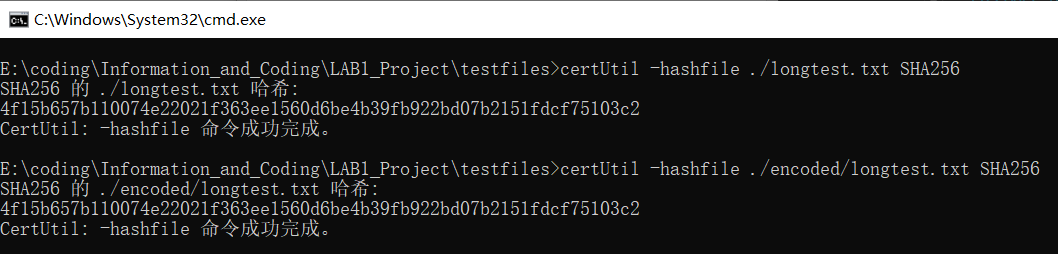
\includegraphics[width=10cm]{./pic/1-2.png}		
    \caption{Huffman编码longtest.txt验证SHA256}
    \end{figure}

    \begin{figure}[H]
    \centering
    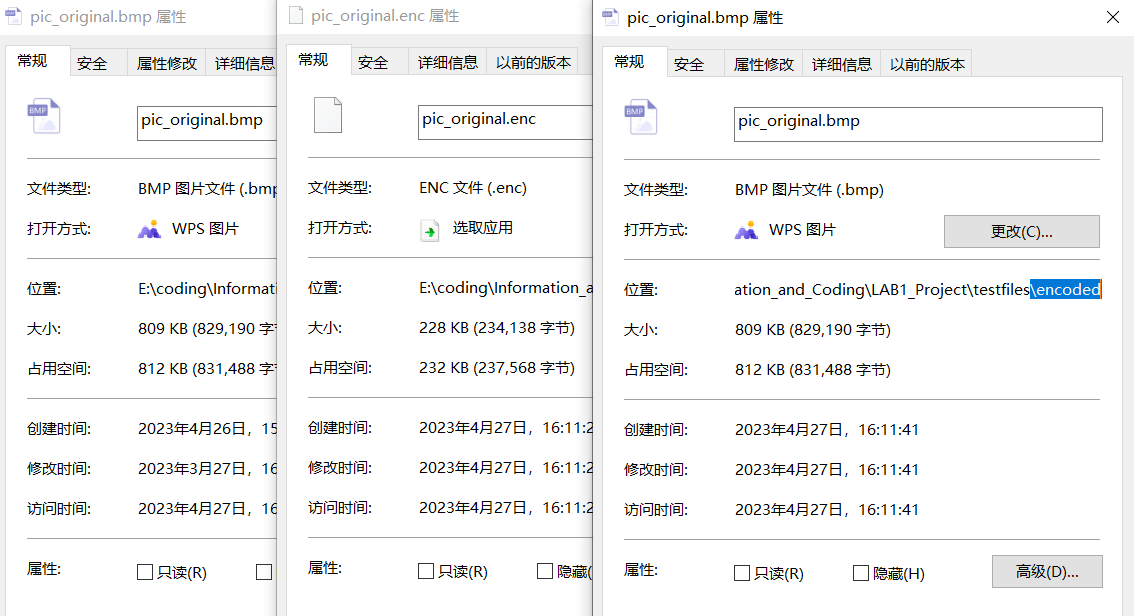
\includegraphics[width=10cm]{./pic/2-1.png}		
    \caption{Huffman编码picoriginal.bmp}
    \end{figure}
    \begin{figure}[H]
    \centering
    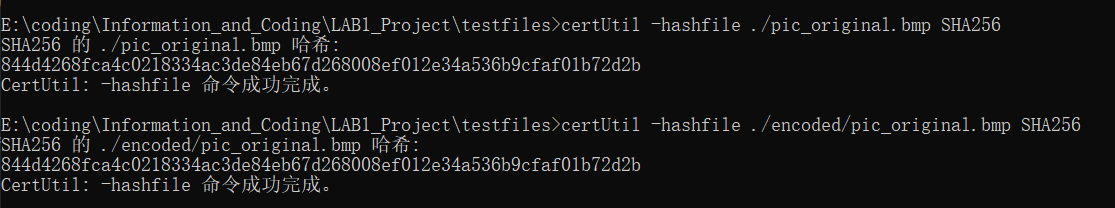
\includegraphics[width=10cm]{./pic/2-2.png}		
    \caption{Huffman编码picoriginal.bmp验证SHA256}
    \end{figure}

    \begin{figure}[H]
    \centering
    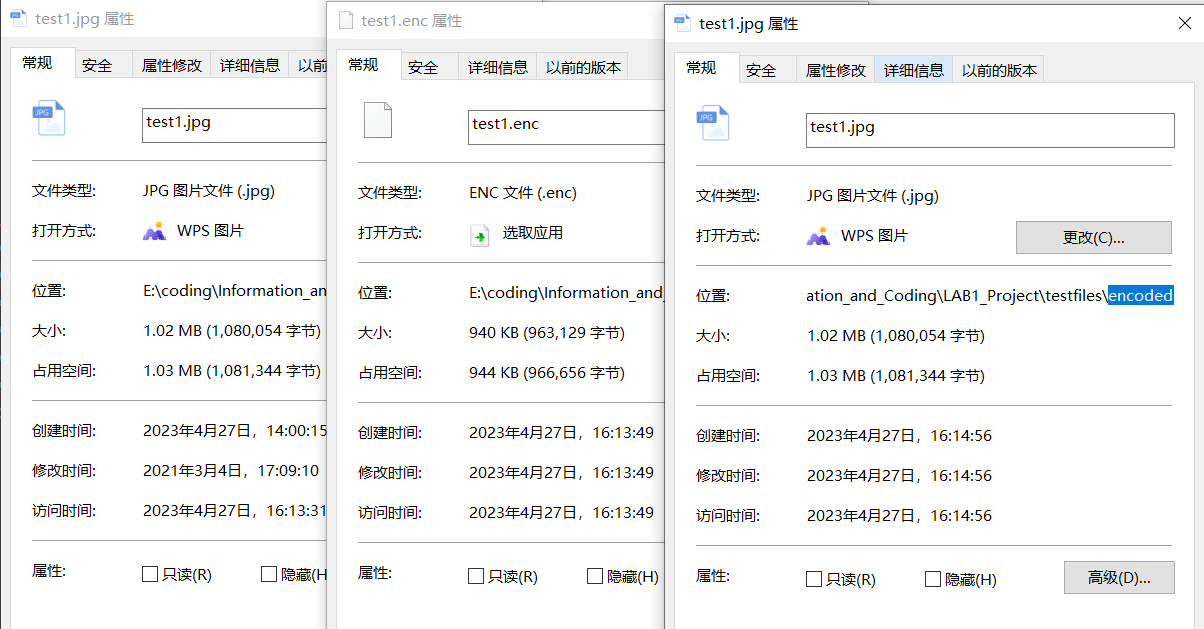
\includegraphics[width=10cm]{./pic/3-1.png}		
    \caption{Huffman编码test1.jpg}
    \end{figure}
    \begin{figure}[H]
    \centering
    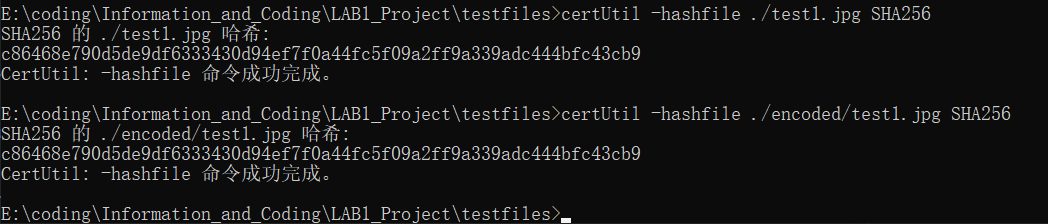
\includegraphics[width=10cm]{./pic/3-2.png}		
    \caption{Huffman编码test1.jpg验证SHA256}
    \end{figure}

    \subsection{用户交互设计}
    
    程序主界面提供编码、解码、编码正确性验证和关于四个选项。
    
    \begin{figure}[H]
    \centering
    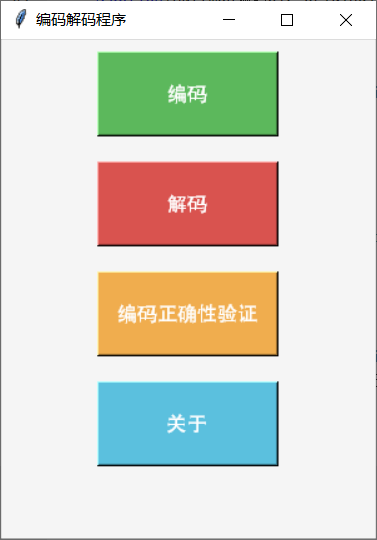
\includegraphics[width=6cm]{./pic/4-1.png}		
    \caption{主界面}
    \end{figure}

    在编码界面可以点击“选择文件”按钮调用系统文件管理器选择文件,也可以手动输入文件路径,编码前会检查路径是否合法。下面提供三个选项,选择对应的编码方式。输出文件的路径默认为待编码文件目录下新建的encoded文件夹。文件名不变,文件类型后缀变为.enc。

    在编码成功过后会返回编码后的文件路径。并显示编码前后的文件大小及编码率。
    
    \begin{figure}[H]
    \centering
    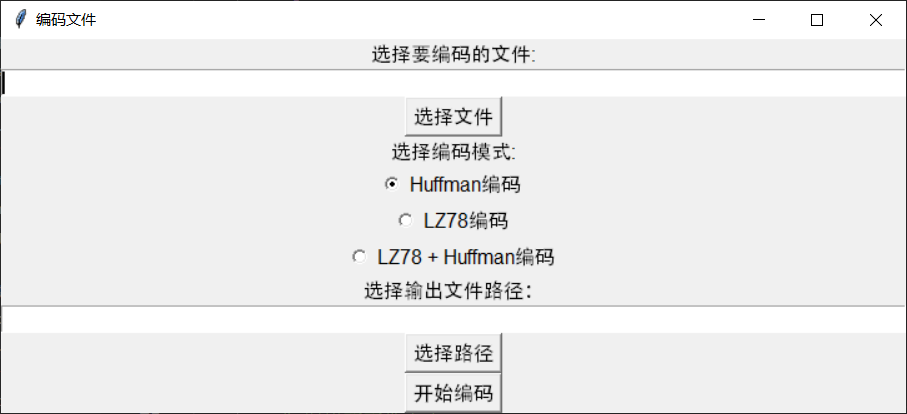
\includegraphics[width=10cm]{./pic/4-2.png}		
    \caption{编码界面}
    \end{figure}
    \begin{figure}[H]
    \centering
    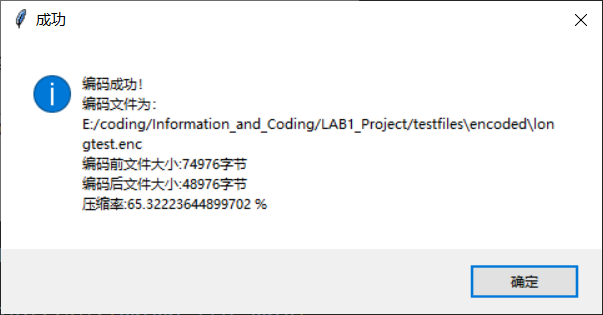
\includegraphics[width=10cm]{./pic/4-3.png}		
    \caption{编码成功}
    \end{figure}

    在解码界面可以选择待解码文件。由于在编码过程中在文件头中存储了是由何种方式编码,因此不需要用户手动选择编码方式,会自动解码。在解码前会检查路径是否合法,文件是否由本程序生成等。输出文件路径默认为待编码文件当前目录,文件名为原文件名,并恢复原文件类型后缀。

    在解码成功后会返回解码文件的文件路径。
    
    \begin{figure}[H]
    \centering
    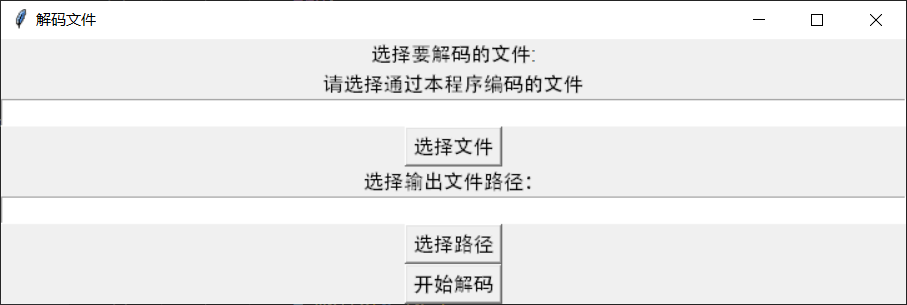
\includegraphics[width=10cm]{./pic/4-4.png}		
    \caption{解码界面}
    \end{figure}
    \begin{figure}[H]
    \centering
    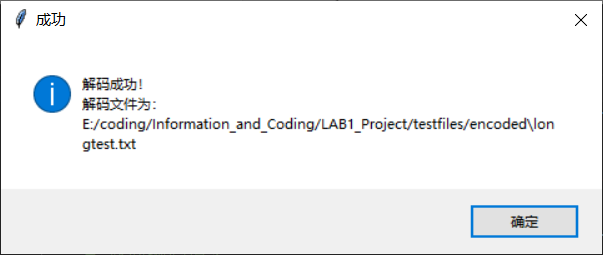
\includegraphics[width=10cm]{./pic/4-5.png}		
    \caption{解码成功}
    \end{figure}

    为了验证编码前源文件和编码和解码后得到的新文件完全相同,在程序中设计了正确性验证功能。在选择一个文件后,在当前目录创建临时文件夹,在临时文件夹中先编码再解码,并自动计算前后两个文件的SHA256哈希值,返回文件编码前后的一致性。
    
    \begin{figure}[H]
    \centering
    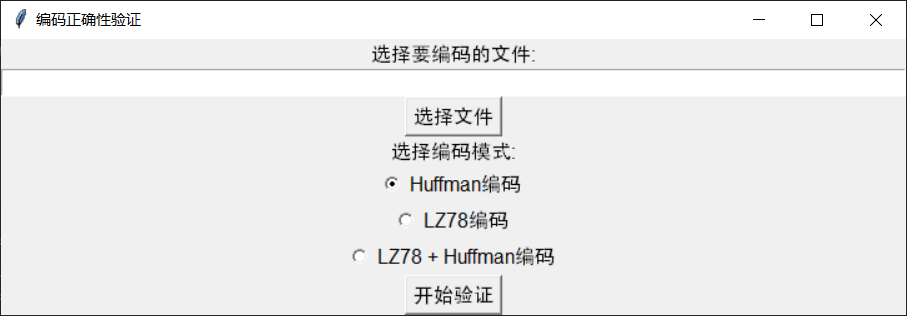
\includegraphics[width=10cm]{./pic/4-6.png}		
    \caption{编码正确性验证界面}
    \end{figure}
    \begin{figure}[H]
    \centering
    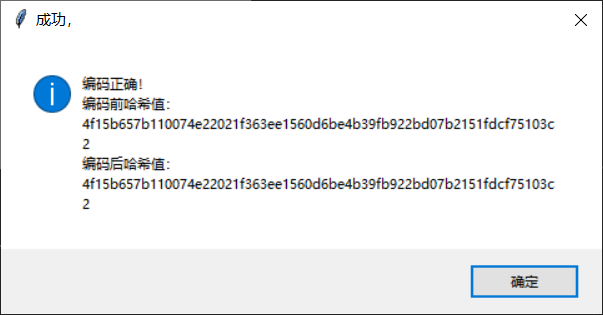
\includegraphics[width=10cm]{./pic/4-7.png}		
    \caption{验证结果}
    \end{figure}

\section{LZ78编码}
    \subsection{代码解释}
    在编码过程中,它通过维护一个字典 treeDict 来存储字符串中出现过的子串,并在遍历字符串时根据字典中已有的子串来输出对应的键值对。当前字符不在字典 treeDict 中时,输出 (0, 当前字符),并将当前字符加入字典 treeDict 中;当当前字符在字典 treeDict 中时,需要寻找以当前字符为开头的最长子串,使得这个子串不在字典 treeDict 中,从而输出 (当前子串的键值, 下一个字符) 并将这个子串加入字典 treeDict 中。

    子串键值所占用的字节数由构建的字典的长度决定,$l = \left \lfloor log_{256}(len(treeDict)) \right \rfloor  + 1$.
    
    在解码过程中,它通过遍历压缩后的列表并根据键值对中的索引和字符来还原原始的字符串,根据字典 treeDict 中对应的键值来构建完整的子串,并将其添加到解压缩后的字符串中。

    LZ78编码过程中没有使用第三方包,使用math的log函数计算字节占用长度。由于使用了函数参数类型与返回值类型的注解,需要Python 3.x 版本。

    \subsection{LZ78编码的基本原理}
    LZ78 的基本原理是将输入的字符串按照子串的重复出现情况进行编码。
    
    具体来说,LZ78 的编码过程中,它维护一个字典,用于存储字符串中出现过的所有子串,初始时字典为空。然后遍历待压缩的字符串,从左至右依次处理字符串的每个字符。
    
    如果当前字符在字典中没有出现过,则将其视为一个新的字符,输出 (0, 当前字符) 并将其加入字典中;如果当前字符在字典中已经出现过,则需要寻找以当前字符为开头的最长子串,使得这个子串不在字典中,输出 (当前子串的键值, 下一个字符) 并将这个子串加入字典中。
    
    在输出时,键值是指已经在字典中出现过的子串在字典中的位置,它是一个整数,可以用更短的编码表示,从而达到压缩的目的。这样,遍历整个字符串后,就得到了一个由键值和字符构成的元组序列,这个序列就是字符串的 LZ78 编码。而在解码过程中,只需要按照相同的规则来还原出原始的字符串即可。
    
    \subsection{安全性和鲁棒性的考虑}
    对于空文件的处理如Huffman编码中所述,在编码前会提示输入为空文件。

    在LZ78编码的最后一个输出中,下一个字符位置可能为空字符。在我的程序中对空字符的处理是不输出,即最后一个输出对只包含子串键值信息。在解码时,通过计算总体的信息长度是否是每对信息长度的倍数,来判断是否需要在最后一个输出对中添加空字符的占位。

    对于使用本程序编码得到的.enc文件,在第一行存储原文件的文件名和文件类型,便于解码过程的恢复,在第二行存储lz字符表示为lz编码得到的,存储lh表示为两个结合编码得到的,并在之后存储其他数据。如果不符合这个格式规范,则会报错提示,此文件并非由本程序编码得到。并且可以通过本标志位在解码时自动判断类型。

    \subsection{结果展示}
    \begin{figure}[H]
    \centering
    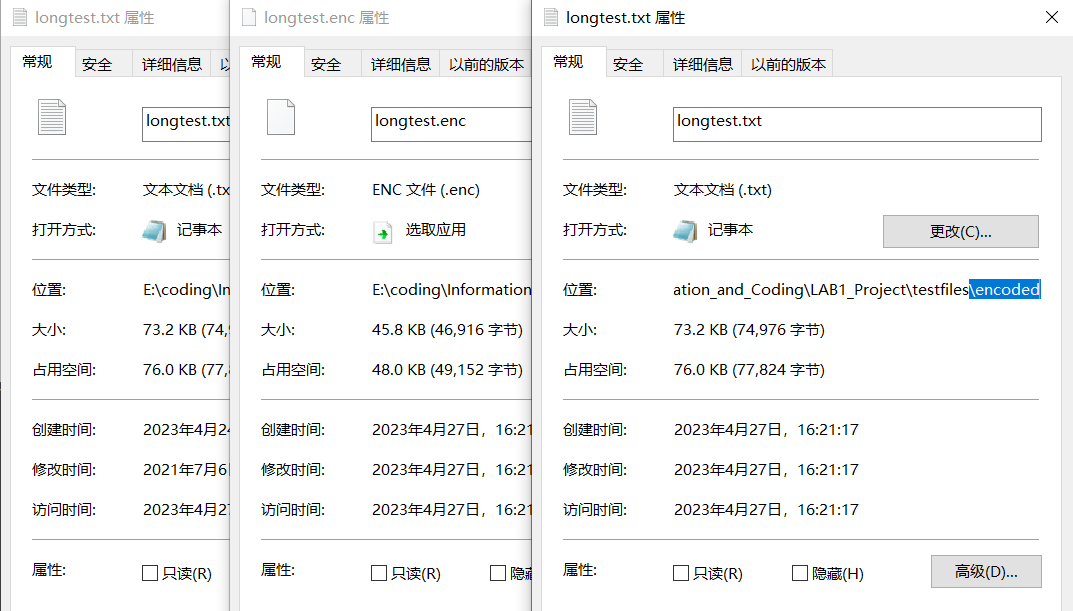
\includegraphics[width=10cm]{./pic/5-1.png}		
    \caption{LZ78编码longtest.txt}
    \end{figure}
    \begin{figure}[H]
    \centering
    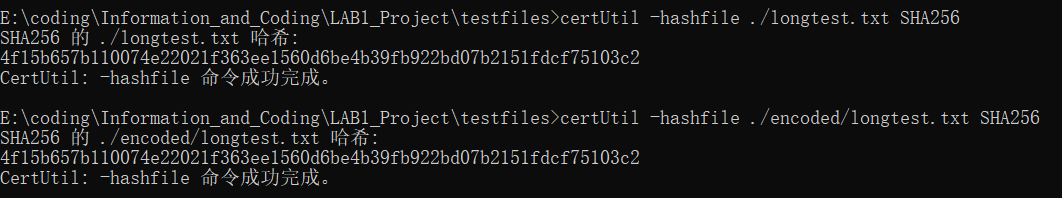
\includegraphics[width=10cm]{./pic/5-2.png}		
    \caption{LZ78编码longtest.txt验证SHA256}
    \end{figure}

    \subsection{用户交互设计}

    在编码页面的编码模式中选择LZ78编码即可以进行编码,其他操作基本一致。
    
    \begin{figure}[H]
    \centering
    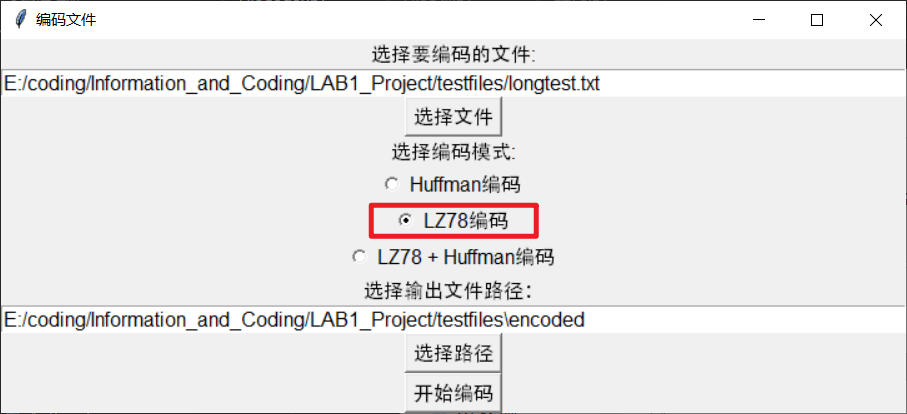
\includegraphics[width=10cm]{./pic/6-1.png}		
    \caption{LZ78编码界面}
    \end{figure}
    \begin{figure}[H]
    \centering
    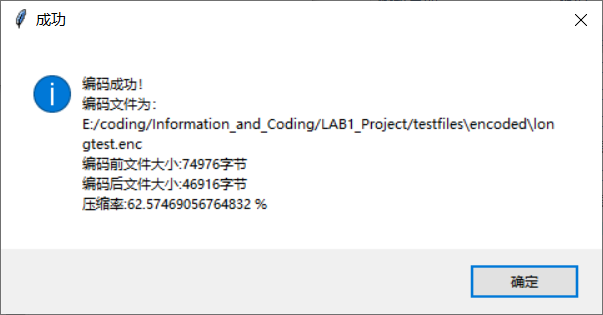
\includegraphics[width=10cm]{./pic/6-2.png}		
    \caption{编码成功}
    \end{figure}

\section{LZ和Huffman结合编码}
    \subsection{结果展示}
    \begin{figure}[H]
    \centering
    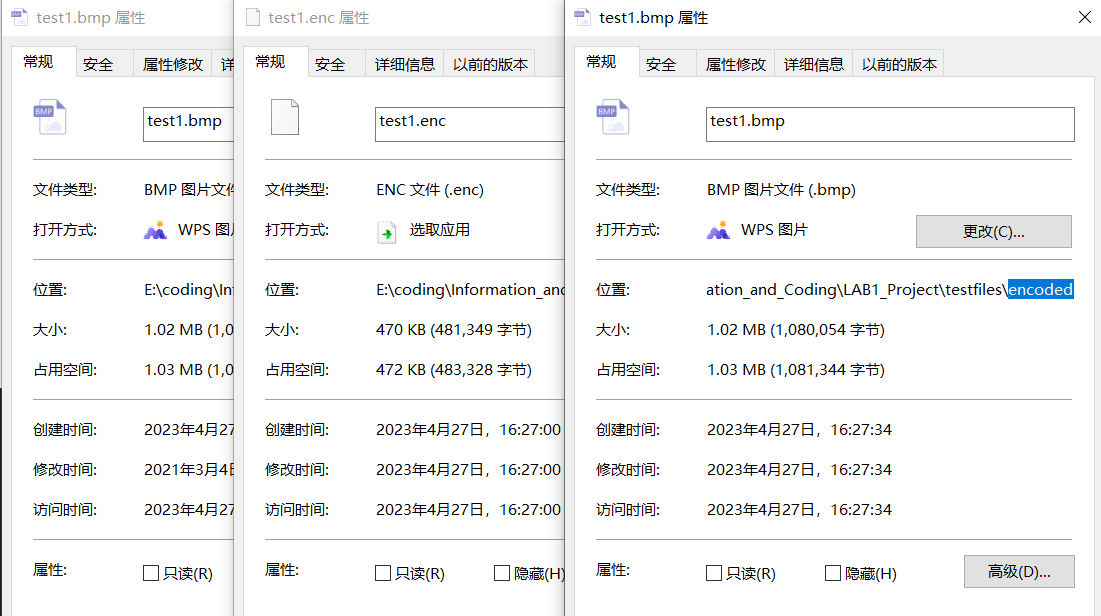
\includegraphics[width=10cm]{./pic/7-1.png}		
    \caption{结合编码test1.bmp}
    \end{figure}
    \begin{figure}[H]
    \centering
    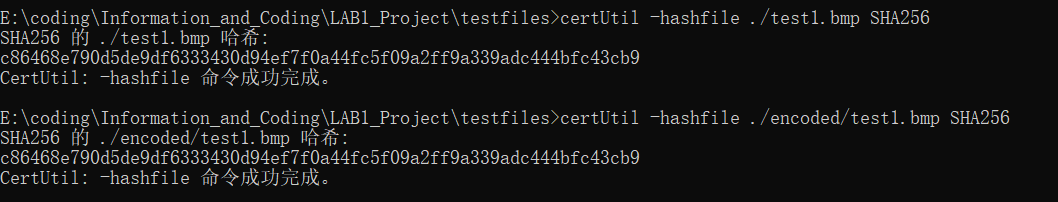
\includegraphics[width=10cm]{./pic/7-2.png}		
    \caption{结合编码test1.bmp验证SHA256}
    \end{figure}

    \subsection{用户交互设计}

    在编码页面的编码模式中选择LZ78+Huffman编码即可以进行编码,其他操作基本一致。
    
    \begin{figure}[H]
    \centering
    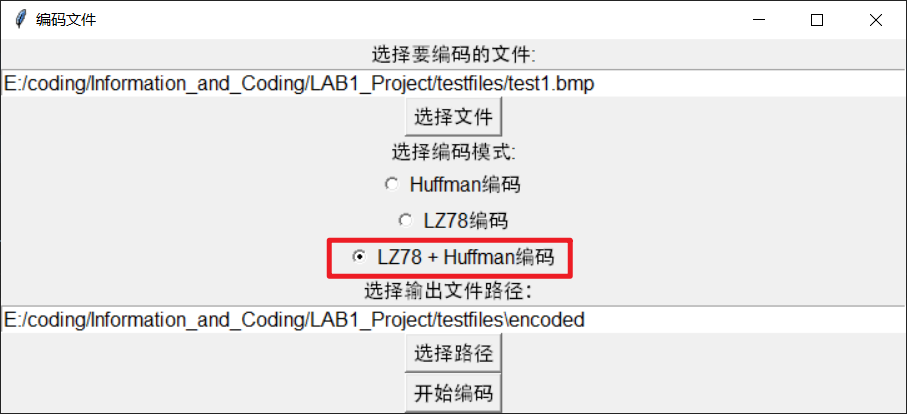
\includegraphics[width=10cm]{./pic/8-1.png}		
    \caption{结合编码界面}
    \end{figure}
    \begin{figure}[H]
    \centering
    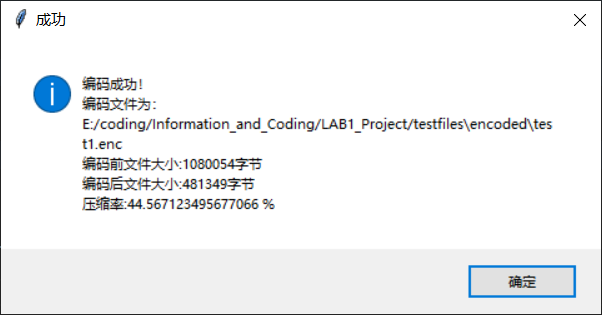
\includegraphics[width=10cm]{./pic/8-2.png}		
    \caption{编码成功}
    \end{figure}
    
    


\section{选做模块 1——重复性的文件结构}

    因为Huffman编码的基本思想是将经常出现的符号编码为较短的比特序列,而较少出现的符号编码为较长的比特序列。在重复性文件结构中,所有符号出现的频率都相同,因此它们将被编码为相同长度的比特序列。由于每个符号都需要相同数量的比特来表示,因此Huffman编码不会提供任何压缩优势;又因为还要存储文件头、码树等相关信息,反而会导致文件变大。
    
    \begin{figure}[H]
    \centering
    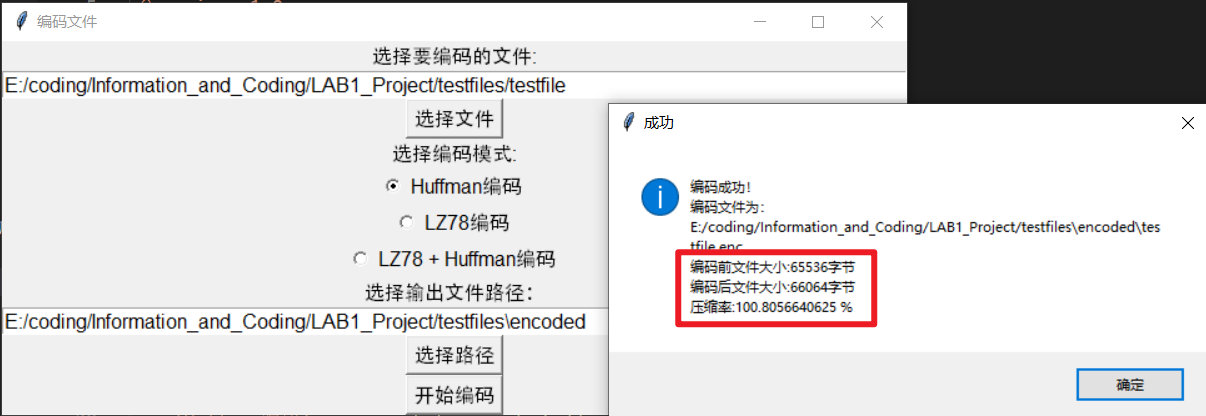
\includegraphics[width=10cm]{./pic/9-1.png}		
    \caption{Huffman编码testfile}
    \end{figure}

    对于具有重复性的文件结构,LZ78编码可以有效地利用这些重复出现的子字符串,将其替换为更短的指针,从而实现数据的压缩。在一个重复性的文件结构中,如果有大量连续的相同字符,LZ78编码可以将这些字符替换为一个指向先前出现的相同字符的指针,从而实现压缩。
    
    \begin{figure}[H]
    \centering
    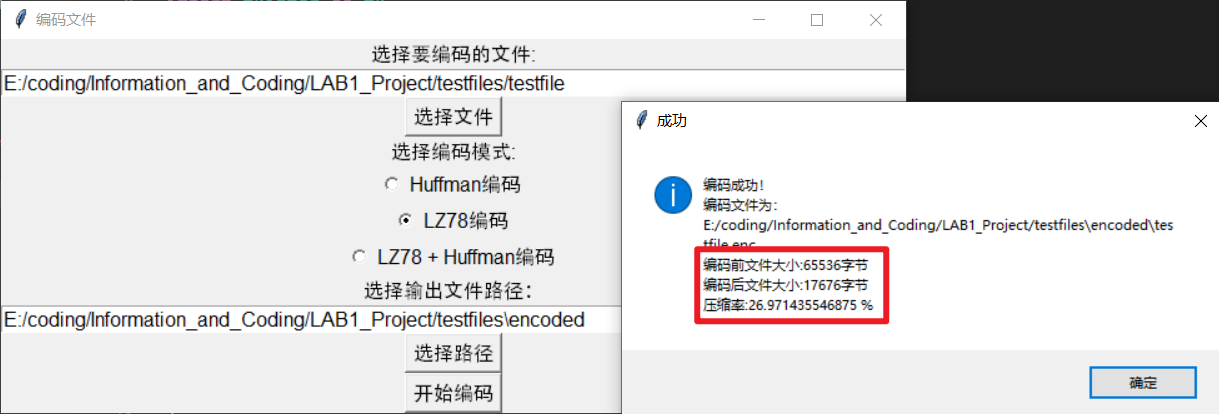
\includegraphics[width=10cm]{./pic/9-2.png}		
    \caption{LZ78编码testfile}
    \end{figure}

\section{选做模块 2——不同格式的压缩}


    BMP格式,图像数据通常以未经压缩的形式存储,因此可以使用Huffman编码和LZ78编码来压缩数据。这些压缩算法可以通过识别重复出现的模式和频率较高的像素值来减小图像数据的存储空间。对于一些具有较多重复模式或较少颜色变化的BMP图像,这些算法可以获得更好的压缩效果。
    \begin{figure}[H]
    \centering
    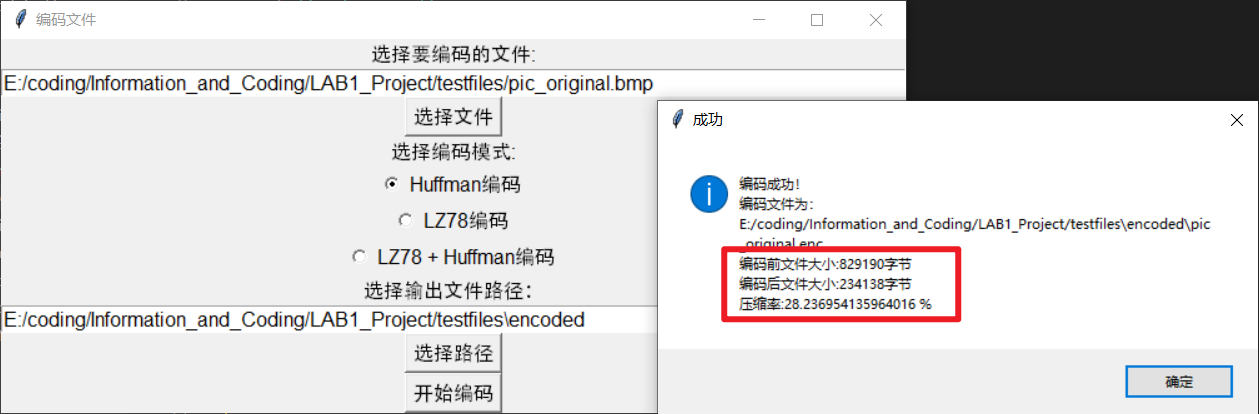
\includegraphics[width=10cm]{./pic/10-1.png}		
    \caption{Huffman编码bmp}
    \end{figure}
    \begin{figure}[H]
    \centering
    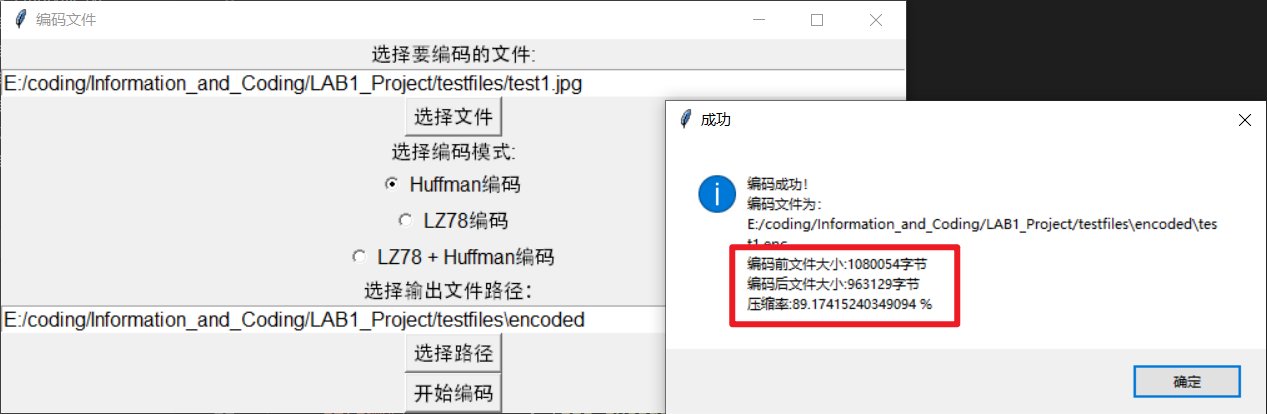
\includegraphics[width=10cm]{./pic/10-3.png}		
    \caption{LZ78编码bmp}
    \end{figure}

    JPEG是一种有损压缩的图像格式,其压缩算法基于变换编码技术和量化。DCT将图像数据转换为一系列频率成分,并使用量化来丢弃较小的频率成分,从而减少图像数据的数量。因此,对于JPEG格式的图像,使用Huffman编码和LZ78编码可能不会产生明显的压缩效果,因为JPEG已经使用了其他压缩技术。
    \begin{figure}[H]
    \centering
    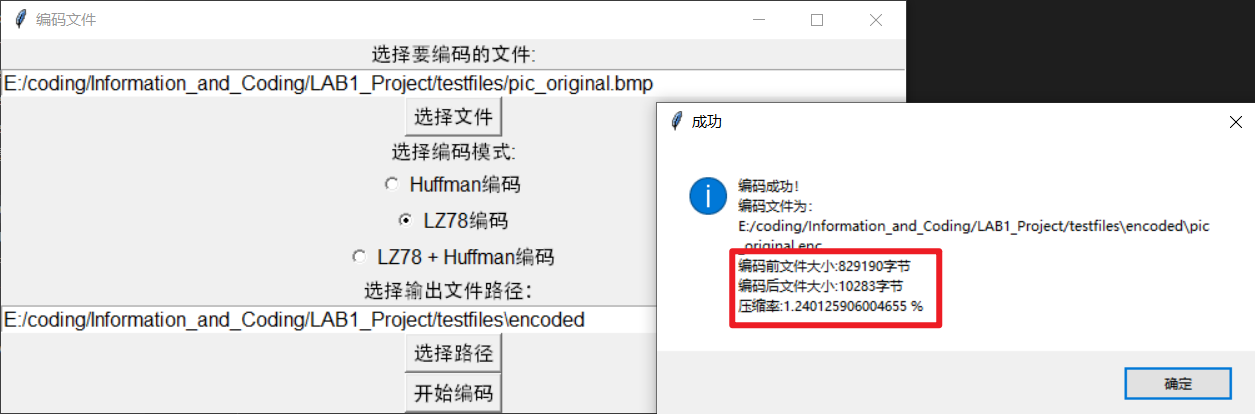
\includegraphics[width=10cm]{./pic/10-2.png}		
    \caption{Huffman编码jpg}
    \end{figure}
    \begin{figure}[H]
    \centering
    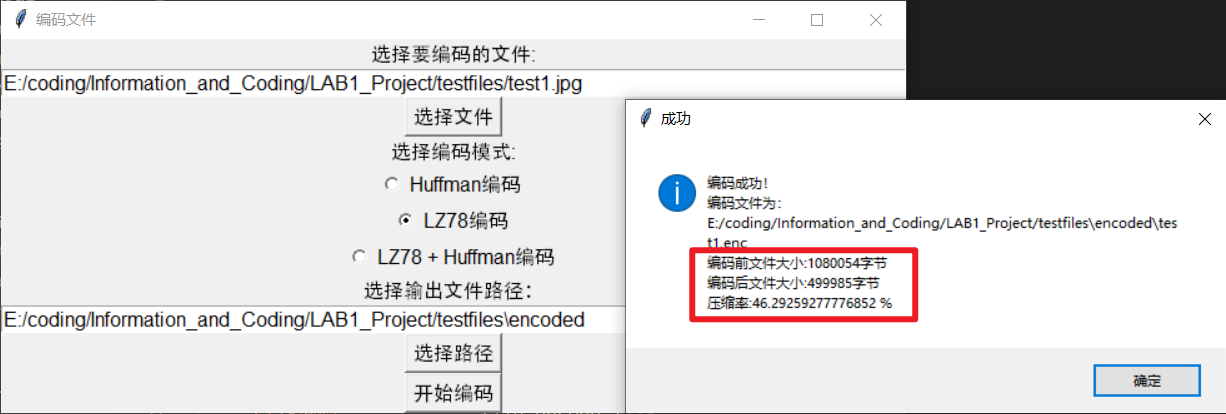
\includegraphics[width=10cm]{./pic/10-4.png}		
    \caption{LZ78编码jpg}
    \end{figure}

\section{选做模块 3——反复压缩}

    \subsection{Huffman编码反复压缩}

    当一个文件被重复压缩时,先前使用Huffman编码所建立的编码表已经包含了原始文件中出现的字符及其频率。如果该文件中包含新的字符,这些字符在先前的编码表中没有出现过,它们的频率将被设置为1,导致编码表的大小增加。同时,如果文件中出现频率较高的字符的位置发生变化,导致其频率增加,编码表的效果也将受到影响。这些因素都可能导致编码表变得不够优化,甚至变得低效,从而导致后续压缩的效果不佳甚至变差。

    
    \begin{figure}[H]
    \centering
    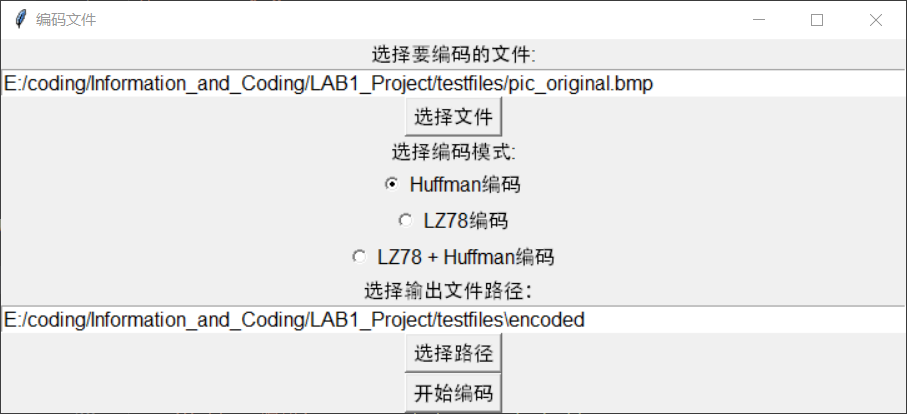
\includegraphics[width=10cm]{./pic/11-0.png}		
    \caption{Huffman编码反复压缩picoriginal.bmp}
    \end{figure}
    
    \begin{figure}[H]
    \centering
    \begin{minipage}[t]{0.45\textwidth}
    \centering
    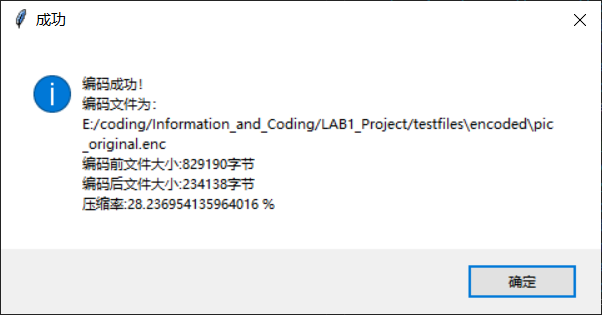
\includegraphics[width=\textwidth]{./pic/11-1.png}
    \caption{Huffman第一次编码}
    \end{minipage}
    \hfill
    \begin{minipage}[t]{0.45\textwidth}
    \centering
    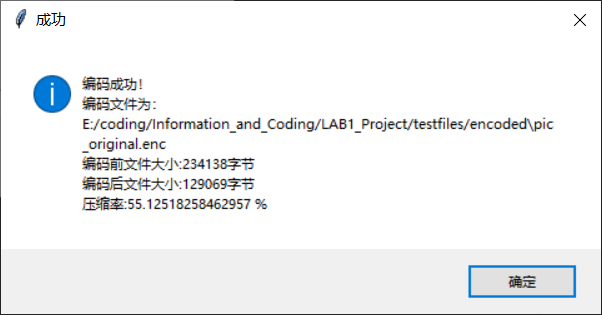
\includegraphics[width=\textwidth]{./pic/11-2.png}
    \caption{Huffman第二次编码}
    \end{minipage}
    \end{figure}

    \begin{figure}[H]
    \centering
    \begin{minipage}[t]{0.45\textwidth}
    \centering
    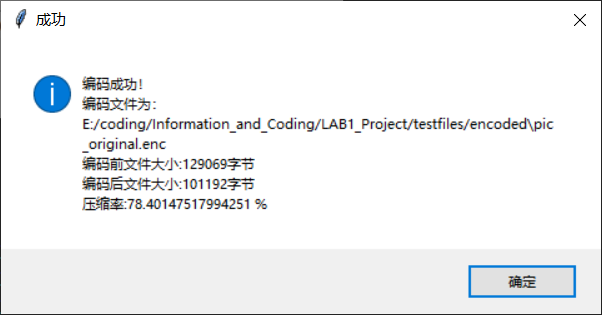
\includegraphics[width=\textwidth]{./pic/11-3.png}
    \caption{Huffman第三次编码}
    \end{minipage}
    \hfill
    \begin{minipage}[t]{0.45\textwidth}
    \centering
    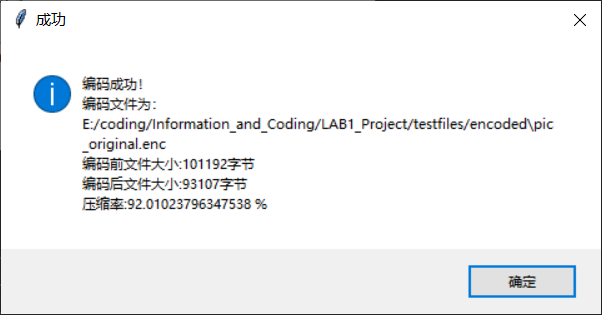
\includegraphics[width=\textwidth]{./pic/11-4.png}
    \caption{Huffman第四次编码}
    \end{minipage}
    \end{figure}

    \begin{figure}[H]
    \centering
    \begin{minipage}[t]{0.45\textwidth}
    \centering
    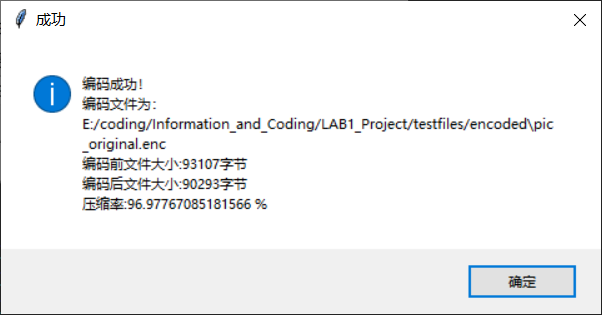
\includegraphics[width=\textwidth]{./pic/11-5.png}
    \caption{Huffman第五次编码}
    \end{minipage}
    \hfill
    \begin{minipage}[t]{0.45\textwidth}
    \centering
    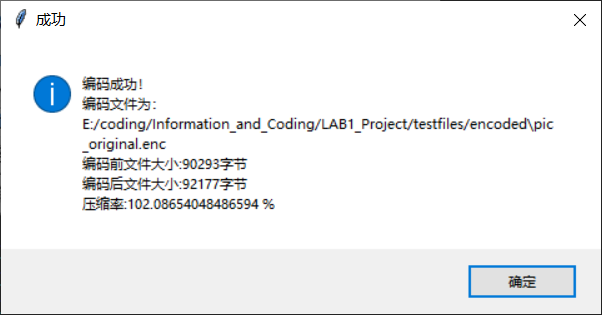
\includegraphics[width=\textwidth]{./pic/11-6.png}
    \caption{Huffman第六次编码}
    \end{minipage}
    \end{figure}


    \subsection{LZ78编码反复压缩}

    当同一个文件被多次使用LZ78编码进行压缩时,前几次压缩的效果通常比较明显,因为在最初的压缩中,词典是空的,而每次压缩后词典都会被扩充。在这个过程中,越来越多的重复序列会被添加到词典中,从而实现更好的压缩效果。

    然而,当同一个文件被反复压缩时,由于压缩后的文件中包含了已经压缩的数据,因此在后续压缩中,LZ78算法需要匹配的序列更加复杂,词典也变得越来越大,这可能导致压缩效果不佳甚至变差。

    \begin{figure}[H]
    \centering
    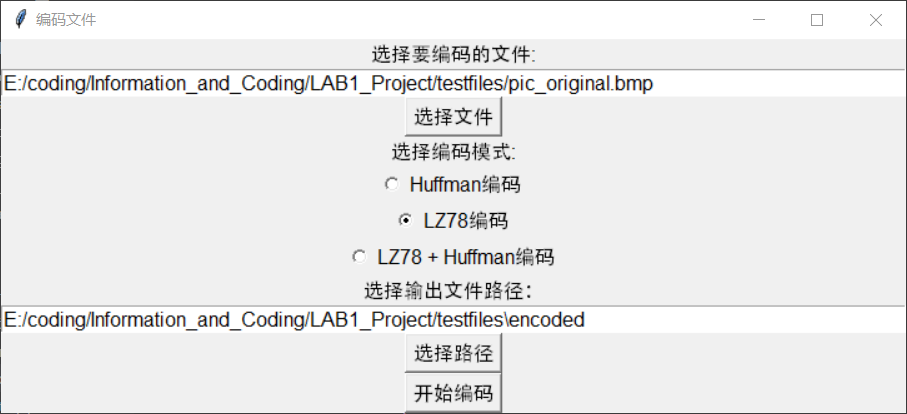
\includegraphics[width=10cm]{./pic/12-0.png}		
    \caption{LZ78编码反复压缩picoriginal.bmp}
    \end{figure}
    
    \begin{figure}[H]
    \centering
    \begin{minipage}[t]{0.45\textwidth}
    \centering
    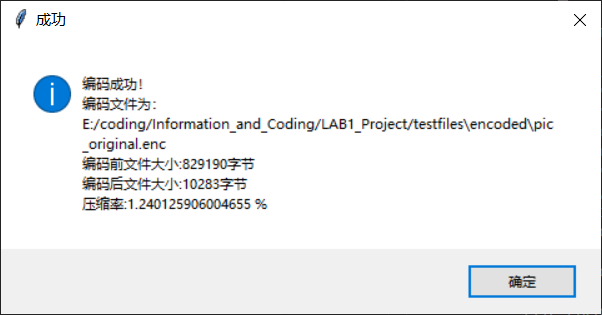
\includegraphics[width=\textwidth]{./pic/12-1.png}
    \caption{LZ78第一次编码}
    \end{minipage}
    \hfill
    \begin{minipage}[t]{0.45\textwidth}
    \centering
    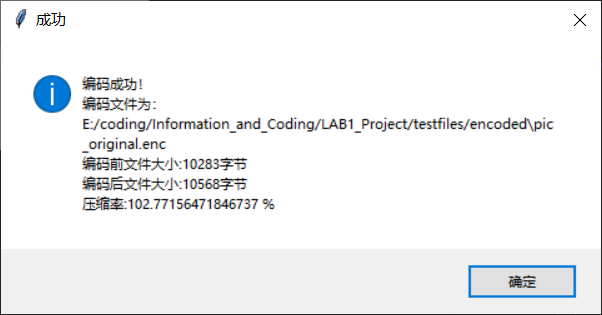
\includegraphics[width=\textwidth]{./pic/12-2.png}
    \caption{LZ78第二次编码}
    \end{minipage}
    \end{figure}

    \begin{figure}[H]
    \centering
    \begin{minipage}[t]{0.45\textwidth}
    \centering
    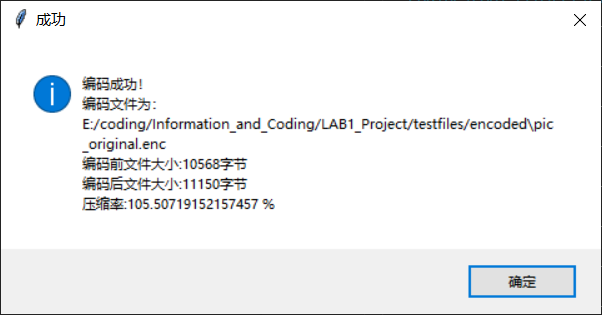
\includegraphics[width=\textwidth]{./pic/12-3.png}
    \caption{LZ78第三次编码}
    \end{minipage}
    \hfill
    \begin{minipage}[t]{0.45\textwidth}
    \centering
    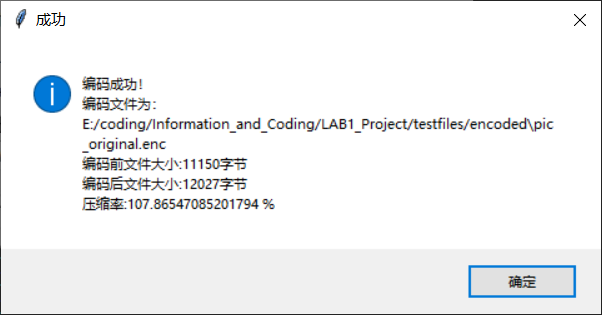
\includegraphics[width=\textwidth]{./pic/12-4.png}
    \caption{LZ78第四次编码}
    \end{minipage}
    \end{figure}

    \begin{figure}[H]
    \centering
    \begin{minipage}[t]{0.45\textwidth}
    \centering
    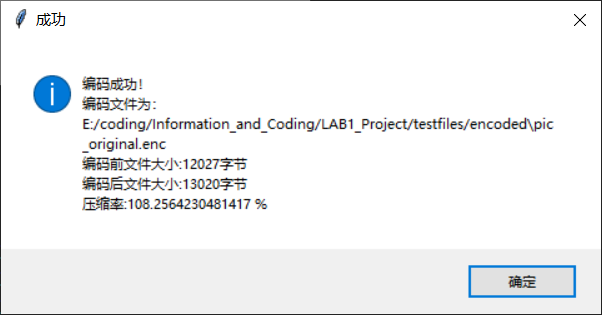
\includegraphics[width=\textwidth]{./pic/12-5.png}
    \caption{LZ78第五次编码}
    \end{minipage}
    \hfill
    \begin{minipage}[t]{0.45\textwidth}
    \centering
    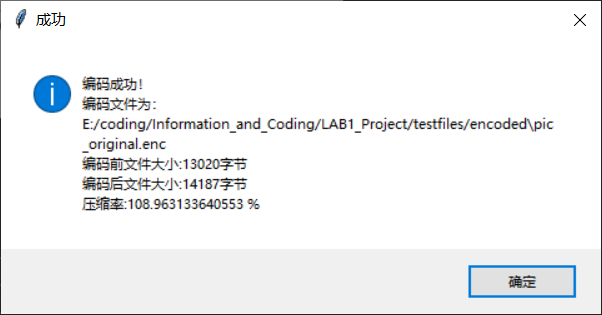
\includegraphics[width=\textwidth]{./pic/12-6.png}
    \caption{LZ78第六次编码}
    \end{minipage}
    \end{figure}

\end{document}